\section{Application: Mobile Privacy\\ Revelations}
\label{sec:characterize-app}

Privacy has rapidly become a critical issue for user interactions with Internet services, particularly in 
mobile environment where location, contact information and other PII are readily available. While the problem 
is well known~\cite{roesner:webtrackers,leontiadis:mobileads,vallina-rod:ads}, previous work lacks a general 
way to identify leaks using network flows alone, and they provide no portable way to block those 
activities. Our key 
contributions are 1) we conduct controlled experiments to identify how PII is being leaked by apps  
 and 2) use \platname{} to understand how this information is being shared both in plaintext and over 
secure channels. 
For our analysis we focus on {\it what} PII is sent,  {\it to whom} is the PII sent, and {\it how frequently} is PII sent.
Then we describe a system that visualizes 
this activity and allows users to block it.

\begin{table*}[t]    
    \centering
    \begin{small}
    \begin{tabular}{|l|l|l|l|l|l|l|l|l|l|}
       \hline
       {\bf Store}&{\bf Platform}&{\bf \# Apps}&{\bf Email}& {\bf Location}& {\bf Name} &{\bf Password}& {\bf Device ID}& {\bf Contacts}& {\bf IMEI}\\
       \hline
       App Store&iPhone&209&13 (6.2\%) &20 (9.5\%)&4 (1.9\%)&6 (2.87\%)&4 (1.9\%)&0 (0\%)&0 (0\%)\\
       \hline
       Google Play&Android&100&3 (3\%)&10 (10\%)&2 (2\%)&1 (1\%)&21 (21\%)&0 (0\%)&13 (13\%)\\
       \hline
Third Party&Android&732&3 (0.4\%)&57 (7.8\%)&3 (0.4\%)&0 (0\%)&85 (11.6\%)&6 (0.8\%)&39 (5.3\%)\\
       \hline
    \end{tabular}
    \end{small}
    \caption{Summary of PII leaked in plaintext (HTTP) by Android and iPhone apps. \emph{The popular iOS apps tend to leak the location information in the clear while Android apps leak the IMEI number and Android ID in the clear. }}
    \vspace{\postfigspace}
    \label{tab:pii}
\end{table*}

\subsection{Controlled experiments}

For our controlled experiments, we created dummy user accounts with fake contact information (see \S\ref{sec:dataset-contr-exper}).  
Our goal is to detect if any PII---email address, phone number, IMEI---stored on the device is leaked across the network over HTTP or HTTPS.
Some of this information is required for normal app operation; however, such information should never travel across the network in plaintext (HTTP).  

\mypara{PII leaks in the clear} 
Table~\ref{tab:pii} presents the PII leaked by Android and iPhone apps. 
The IMEI, a unique identifier tied to a mobile device, and the Android ID (tied an Android installation) are the most commonly leaked PII by Android apps.  
These can be used to track and correlate a user's behavior across Web services. 
Table~\ref{tab:pii} shows that other information like contacts, emails, and passwords are also leaked in the clear. 
The email address used to sign up for the services was leaked in the clear by 13 iOS and 3 Android apps from our set of popular apps.
While only one Android app (belonging to the \emph{Photography} category) leaked a password in the clear, we were surprised to learn that six of the most popular iOS apps send user credentials in the clear, \emph{including the password}. 

Particularly disconcerting is our observation that an app in the Medicine category -- which the provider claims has ``\emph{1 million active members 
of which 50\% are US physicians}'' -- sends the user's first name, last name, email, password, and zip code in the clear. 
Given US physicians have access to highly sensitive data like medical records, we believe it is particularly important for this app to protect user credentials (which are often used for multiple services). 

\mypara{PII leaked from same apps on different OSes} 
We observed that the information leaked by an app depends on the OS.
Of the top hundred apps for iOS and Android, 26 apps are available on both iOS and Android. 
Of these 26 apps, 17 apps leaked PII on at least one OS: 12 apps leaked PIIs only on Android, 2 apps leaked PII only on iOS, while only one app had the same data leakage in both OSes.
Of the remaining two apps that leaked PII, one app leaked the android ID and IMEI in Android and username in iOS, while the other app leaked the Android~ID in Android and location in iOS. 
This observation, the dependence of PII leaks on the OS, highlights the importance of \meddle that can analyze PII leaks across multiple OSes.

\begin{table}
    \centering
    \begin{small}
    \begin{tabular}{|l|c|c||c|}
       \hline
       {\bf Host}& {\em Ads \& Analytics} \tabularnewline
       \hline              
       android.clients.google.com & -  \tabularnewline
       getjar.com        & -  \tabularnewline
       chartboost.com    & \checkmark \tabularnewline
       pocketchange.com  & -   \tabularnewline
       flurry.com        & \checkmark \tabularnewline       
       \hline
    \end{tabular}
    \end{small}
    \caption{\textbf{Top 5 domains that receive PII over SSL ordered according to number of flows leaking PIIs during controlled experiments}. \emph{Two of the top 5 hosts that receive this information is an ads and analytics site.}}
    \label{tab:pii-leakage-https-sites}
    \vspace{\postfigspace}
\end{table}

\mypara{PII leaked over SSL} 
During our experiments, we observed that PII is also sent over HTTPS. 
We observe that two of the top 5 sites  that receive this information are ads and analytics (A\&A) sites.

Our observations highlight the limitations of current mobile OSes with respect to controlling access to PII via app permissions. 
In particular, it is unlikely that users are made aware that they are granting access to PII for A\&A sites when embedded in an app that serves a different purpose. 
This problem is pervasive: of the 77 sites that received some PII in the clear or over HTTPS, 35 sites were third party ads and analytics sites.

We note that our observations are a conservative estimate of PII leakage. 
Specifically, we cannot detect PII leakage if the data is obfuscated (\eg via hashing). 
Regardless,  our study shows that a significant amount of PII leaks not only through unobfuscated channels but even unencrypted ones. 

\subsection{PII in the Wild}

We now analyze the \mobWild{} dataset. 
Note that we do not use SSL bumping on this data for privacy reasons. 

\noindent\textbf{Location leaks.} We observe that a bus service app (\emph{One Bus Away}), the
app that manages the iOS homescreen (\emph{SpringBoard}), and
weather apps (\emph{TWC}, \emph{Weather}, and \emph{Hurricane})
were responsible for more 78\% of the flows that sent the location
information in the clear. Other apps that do not require location information, 
such as YouTube, Epicurious and EditorsChoice, also leaked GPS coordinates.
Further, \emph{SpringBoard} sends location information in the clear to fetch weather information from Yahoo servers. 
We observe that \emph{SpringBoard} leaked location information for 11 devices in the \mobWild dataset, a maximum of 14 leaks per day was observed for one device, sufficient to expose a user's daily movements to anyone tapping Internet connections~\cite{nsa:globaltracking}. 

\noindent\textbf{Unique ID leaks.} 
The device ID and IMEI are frequently leaked in the clear, and as in the case of controlled experiments, A\&A sites are the most popular destination for the IMEI leaks.  
Among the 16 sites that received  these unique IDs in the clear, 10 are A\&A sites; the rest of the sites includes sites for games, news, and manufacturer updates.

\begin{table}
\centering
\begin{small}
\begin{tabular}{|p{0.35\columnwidth}|p{0.1\columnwidth}|p{0.15\columnwidth}|p{0.1\columnwidth}|}
\hline
\multirow{2}{*}{\bf Tracker} & \multicolumn{3}{c|}{\bf Number of devices tracked}\tabularnewline
\cline{2-4}
                      &  {\bf Total} & {\bf iOS} & {\bf Android} \tabularnewline
\hline
doubleclick.net       & 26 {\em(all)} & 15 {\em(all)} & 11 {\em(all)} \tabularnewline
\hline
google-analytics.com  & 26 {\em(all)} & 15 {\em(all)}  & 11 {\em(all)} \tabularnewline
\hline
googlesyndication.com & 22 & 12 & 10 \tabularnewline
\hline
admob.com             & 21 & 11 & 10 \tabularnewline
\hline
scorecardresearch.com &  21 & 11 & 10 \tabularnewline
\hline
\end{tabular}
\end{small}
\caption{The top 5 ads and analytics sites that were contacted by the devices in our dataset.
\emph{All 26 devices in} \mobWild \emph{contacted doubleclick.net and google-analytics.com}.}
\vspace{\postfigspace}
\label{tab:top-trackers}
\end{table}

In Table~\ref{tab:top-trackers}, we present the number of devices in the \mobWild dataset that contact the most popular A\&A sites.
We observe that all the devices in the \mobWild dataset contacted doubleclick.com, an ad site, and google-analytics.com, a tracking site. 
Further, 66.12\% of the ads and analytics traffic volume in the \mobWild dataset contained the default OS \useragent or the user agent of browsers, 6.46\% of the traffic contained a blank user-agent field, and 4.8\% of the traffic contained a signature of \emph{Google-Analytics} library.
The rest of the traffic contained signatures of other apps such as Facebook, Pandora, and YouTube.

\subsection{Revealing and Controlling PII Leaks}
\label{subsec:recon}

Given the extensive nature of tracking over mobile devices, we developed  
\emph{ReCon}, a tool to visualize how user's are being tracked as they use their devices. 
\emph{ReCon} provides a visual interface similar to Mozilla Collusion~\cite{collusion}; instead of 
visualizing only websites, our tool shows apps and the 3rd party sites they contact. Figure~\ref{fig:recon} shows screen captures of our tool, with the default view of trackers contacted by apps (left) and how 
hovering/tapping on a tracker reveals the apps contacting the tracker (right). Similarly, hovering/tapping on an app 
highlights all the trackers contacted by the app.

\begin{figure}[tb]
\subfloat[Default view.]{\label{fig:recon-all} 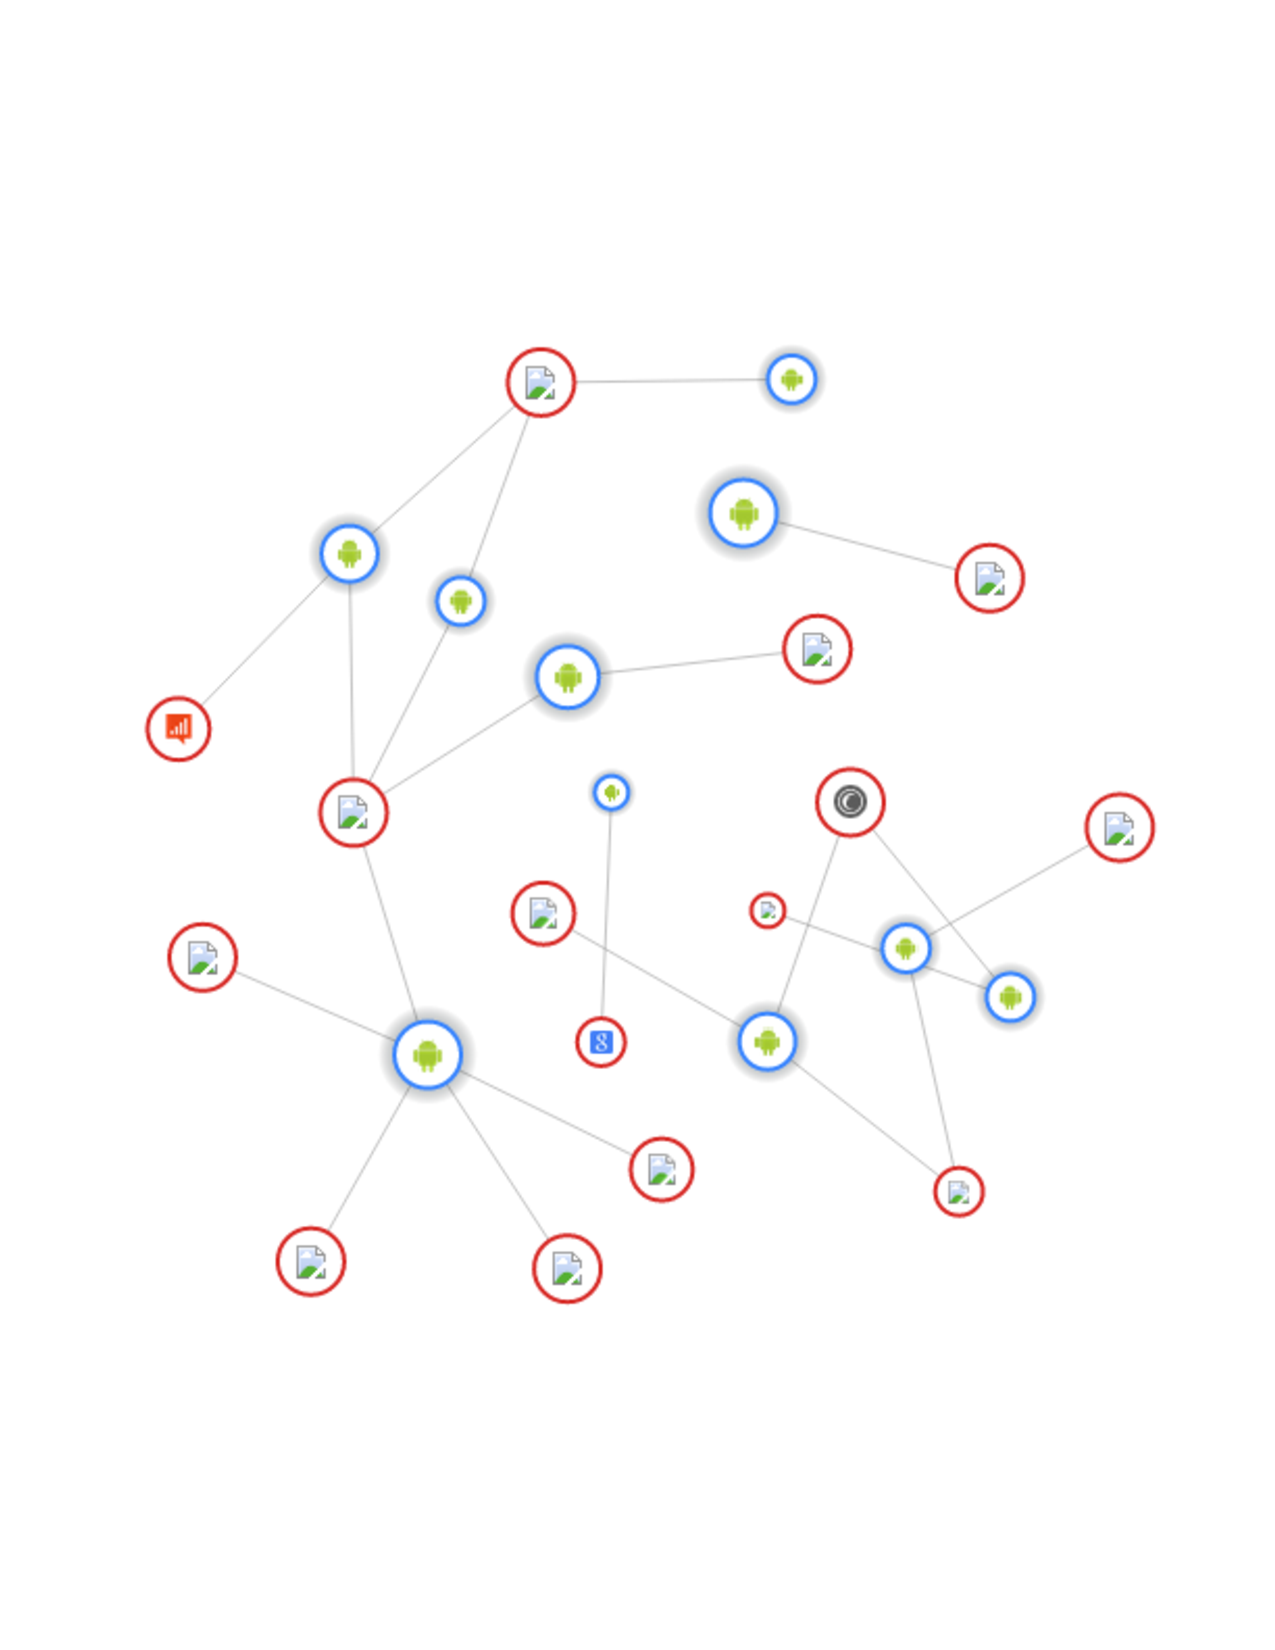
\includegraphics[width=0.47\columnwidth]{figures/ReConAll.pdf}}
\hspace{0.1in}
\subfloat[View showing tracking by Scorecard Research.]{\label{fig:recon-highlight} 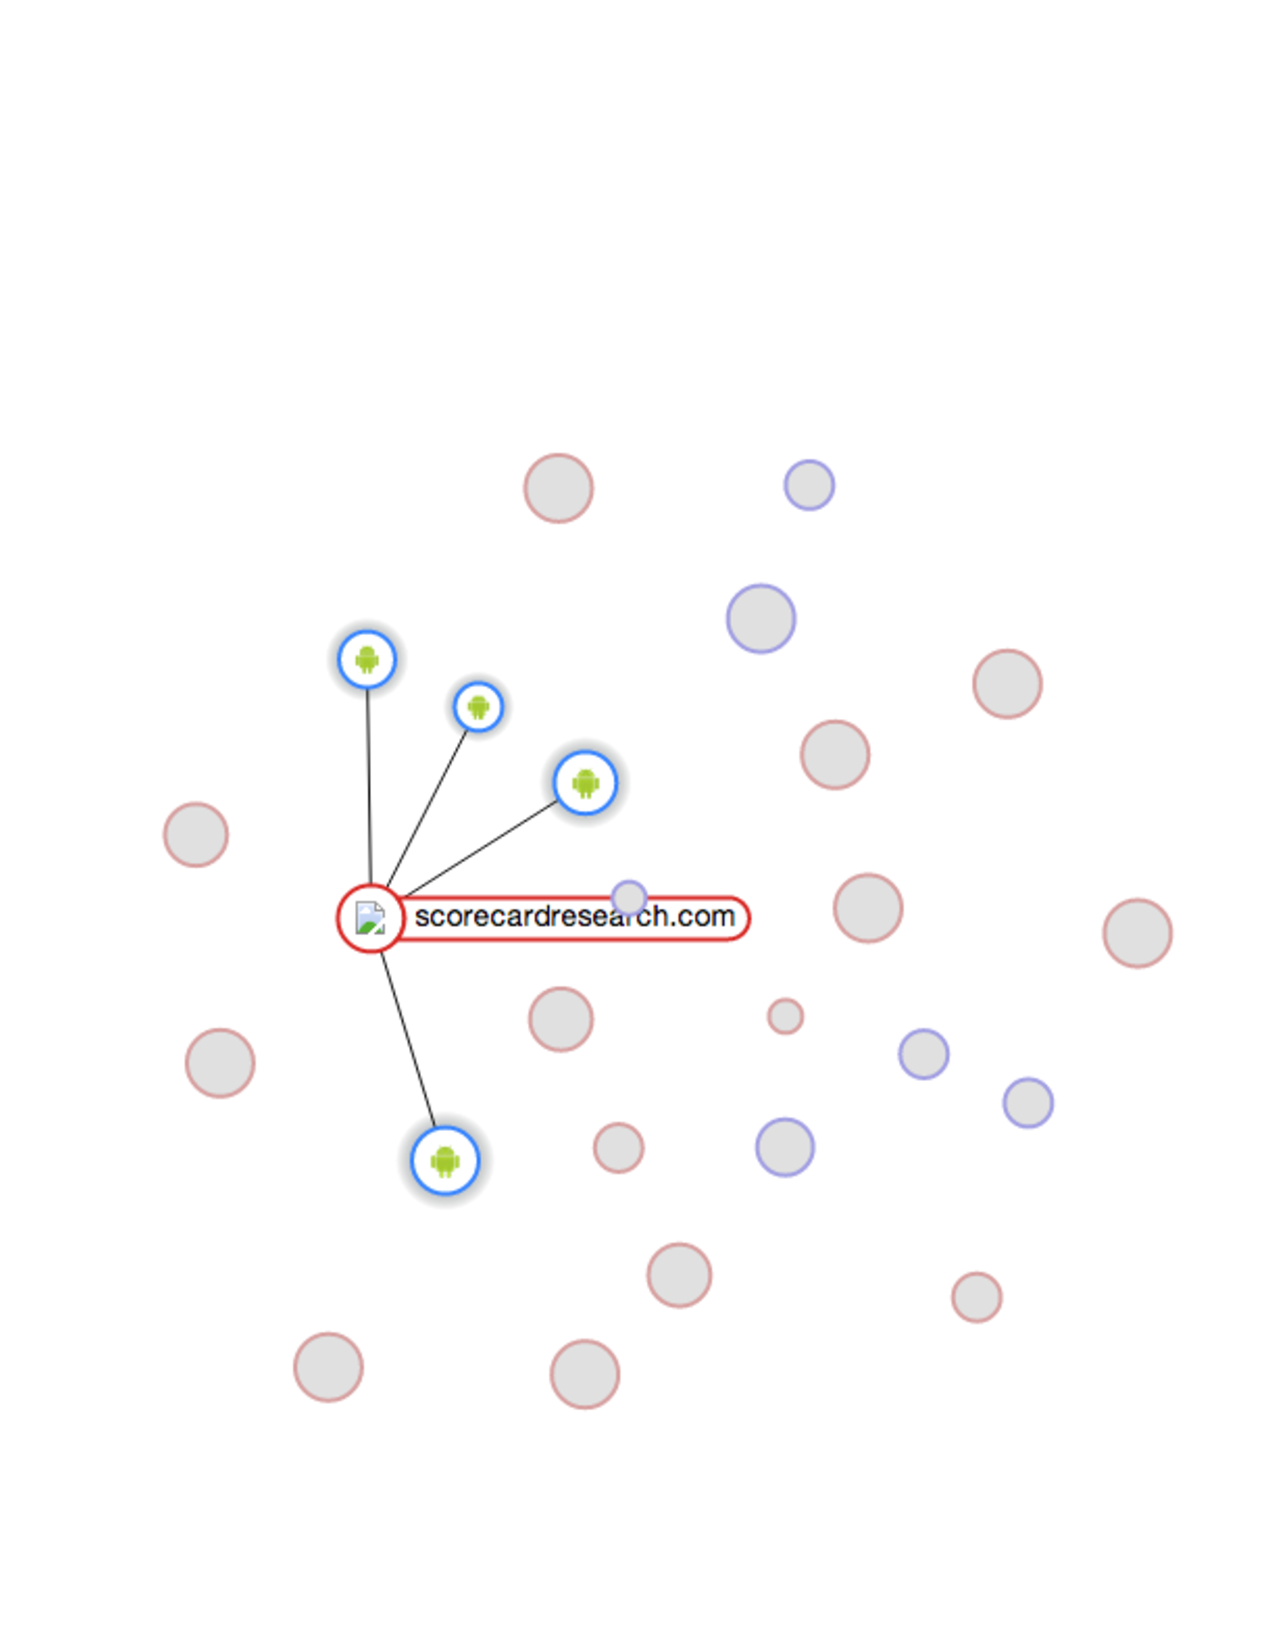
\includegraphics[width=0.47\columnwidth]{figures/ReConHighlight.pdf}}
\caption{Screen captures of the \emph{ReCon} tool, allowing users to visualize how they are being tracked by apps, and install custom filters by clicking on links to ``remove'' them. }
\label{fig:recon}
\vspace{\postfigspace}
\end{figure}

In addition to revealing privacy leaks, \emph{ReCon} allows users to block them. Specifically, users can 
click/tap on a link to ``destroy'' it -- installing a custom 
filter for the corresponding (app, tracker) pair. To make this approach practical, we are developing 
an interface to crowdsource block lists, much like how Web browser ad-blocking filters are maintained 
and distributed. A demo of our tool is located at \url{http://goo.gl/A17h9}. \drc{Update this link}


%%% Local Variables: 
%%% mode: latex
%%% TeX-master: "main"
%%% End: 

%       getjar.com     & - S & - S \tabularnewline
%       aarki.net      & - S & - - \tabularnewline
%       chartboost.com & - S & - S \tabularnewline
%       *pocketexchange&   S &   S \tabularnewline
%       *vserv.mobi    & - - & C   \tabularnewline
%       *groupon.com   &     &   S
%       *flurry.com    &     &   S
%       *bankofamerica &     &   S
%       *google.com    & - - & - S

%\section{MISC}

% \begin{figure}
% \centering
% \includegraphics[width=\columnwidth]{plots/ads_wild_gatracking.pdf}
% \caption{Number of devices tracked by Google-Analytics. \emph{We observe that devices }}
% \label{fig:tracking-analytics}
% \end{figure}

% \begin{figure}
% \centering
% \includegraphics[width=\columnwidth]{plots/ads_wild_usertracking.pdf}
% \caption{Number of sites that track a user. \emph{We observe that devices }}
% \label{fig:tracking-analytics}
% \end{figure}

% \begin{figure}
% \centering
% \includegraphics[width=\columnwidth]{plots/ads_wild_sitescontacted.pdf}
% \caption{Number of visits to A\&A sites per device. \emph{The error bars indicate the 25$^{th}$ and 75$^{th}$ percentiles. Each visit is a potential tracking visit.}}
% \label{fig:tracking-analytics}
% \end{figure}

% \begin{table}    
%     \centering
%     \begin{small}
%     \begin{tabular}{|l|c|c|}
%        \hline
%        {\bf Host}&{\bf IMEI}&{\bf Device ID}\tabularnewline
%        \hline              
%        tapjoyads.com  & Y & - \tabularnewline
%        zynga.com      & Y & - \tabularnewline
%        iheart.com     & Y & Y \tabularnewline
%        google.com     & - & Y \tabularnewline
%        flurry.com     & - & Y \tabularnewline
%        \hline
%     \end{tabular}
%     \end{small}
%     \caption{Hosts to which the IMEI or Device ID was sent in the clear and over HTTPS. \emph{The value Y for a column implies that data was sent over HTTP and HTTPS. We order these hosts based on the number of flows that sent the IMEI number in the clear and over HTTPS.}}
%     \label{tab:pii-leakage-sites}
% \end{table}

%Moreover, we observe that 4\% of the flows
%sent the location information to ads and analytics sites; the rest of the
%flows being from apps including browsers, the Facebook app, and angry birds. 
% more than
%80\% of \emph{ad-flows} leaking location information did not include
%an application signature in the user-agent field, 
%Similarly, from the device of one of the authors of the paper, we observed that the latest three versions YahooMail application, up to the time of the measurements, leaked the user's email address in the clear.


%\tbd{This should come before 
%We first identify A\&A flows using the publicly available database of~\cite{YoyoAds}; we augment this list of domains using recent research on mobile ads~\cite{hornyack:appfence, leontiadis:mobileads}.
%Based on this classification, we observe that the ads and analytics traffic was responsible for up to 6\% of the traffic by volume per device, an observation in line to the one made by Vallina-Rodriguez~\etal~\cite{vallina-rod:ads}}.

%\subsection{Ads and Analytics in the Wild}

% \tbd{focusing on ads and analytics is just what you did in the
%   previous paragraph. What is new or different in this one.}
% We now focus our attention on the extent to which devices in the
% \mobWild dataset contact ads and analytics (A\&A) sites, an activity
% that is receiving considerable
% attention~\cite{roesner:webtrackers,leontiadis:mobileads,vallina-rod:ads}.
% Using our classification based on the \httphost, we observe that the
% ads and analytics traffic was responsible for up to 6\% of the traffic
% by volume per device, an observation in line with the one made by
% Vallina-Rodriguez~\etal~\cite{vallina-rod:ads}.  Rather that focusing
% on the traffic volume we focus on the extent to which these sites are
% able to track the users in the dataset and the applications that
% facilitate this tracking.
%\tbd{This must come before Furthermore, we observed that 7\% of the traffic contained the Google-Analytics in the signature field; this signature was observed even in the flows for users that did not have the Google Analytics application installed on the device. Mention that we will wrongly classify the flows from Google Analytics app as ads and analytics traffic} 

%In summary, we use our controlled experiments to identify PII leaks on
%both HTTP and HTTPS, and we show that PII are leaked to third party
%sites such as ads and analytics. These controlled experiments are a
%practical use case of \platname, experiments requiring warranty
%voiding the devices otherwise. In particular, \platname{} enable to
%reveal PII leaks over HTTPS.
%However, we would like to point out that we were not able to analyze traffic in which the data sent was encoded and exchanged as binary objects. 

%Stats value 13 of 22 in the clear device ID, 16 of 39 IMEI clear,  3 of 6 IMEI HTTPs, 3 of 10 device HTTPs}

%In this section we describe how we use \meddle to identify privacy leaks and tracking by third parties 
%in mobile systems. While previous work identifies many of the same issues, they lack a general 
%way to identify leaks using network flows alone, and they provide no portable way to block those 
%activities. In the following sections, we describe how we identify the apps responsible for privacy 
%leaks and tracking, regardless of whether they use SSL. Then we describe a system that visualizes 
%this activity and allows users to block it.
%
%
%\subsection{Identifying Privacy Leaks}

%To answer these questions, we rely on the controlled experiments and the \mobWild dataset.

%We evaluate PII in terms of two threat models. First, we assume a passive eavesdropper that can sniff 
%traffic over open WiFi APs or within a cellular provider. Any PII sent unencrypted is available to the attacker. 
%Second, we assume an attack conducted by (or on) a third-party service that is able to identify a user's fine-grained locations 
%over time. 

%TuneIn Player leaked the device location.
%Another two apps both leaked data, but different types: Snapchat leaked Android ID and IMEI but leaked username in iOS and Brightest Flashlight leaked Android ID and leaked location in iOS. Two apps leaked PII only in iOS (Groupon and Pandora), while 12 apps leaked data only in Android. Most Android leaks were  Android ID; however, 4 of these apps leaked location and 1 leaked IMEI. For the top apps, Android leaks more PII than iOS.

% For your eyes only ;)
%services.epocrates.com  Mozilla/5.0 (iPhone; U; CPU iPhone OS 4_0 like Mac OS X; en-us) AppleWebKit/532.9 (KHTML, like Gecko) Version/4.0.5 Mobile/8A293 Safari/6531.22.7   1370172894.1735 JXMXaFcr2Pd 10.11.4.52  55904   63.241.66.139   80  7   GET /userprofile/userprofile/userprofile/userprofile?datatype=json&os=6.1.3&device_model=iPhone&appVersion=5.2&appId=nc-2&data={"countryId":"10","lastName":"Test","firstName":"Meddle","password":"epocratespwdW1","passwordConfirm":"epocratespwdW1","email":"mailmeddle@yahoo.com","occupationId":"56","zipCode":"98105"}&action=useraccount&platform=14&subaction=createuser    -   0   40001   200 OK  -   -   -   (empty) -   -   -   text/plain  -   -   -   0       -   -   shen

% \begin{table}
%     \centering
%     \begin{small}
%     \begin{tabular}{|l|c|c||c|}
%        \hline
%        {\bf Host}&{\bf IMEI}&{\bf Device ID} & {\em Ads \& Analytics} \tabularnewline
%        \hline              
%        chartboost.com                & \checkmark & \checkmark & \checkmark  \tabularnewline
%        tapjoyads.com                 & \checkmark & -          & \checkmark  \tabularnewline
%        getjar.com                    & \checkmark & \checkmark & -   \tabularnewline
%        pocketchange.com              & \checkmark & \checkmark & -   \tabularnewline
%        iheart.com                    & \checkmark & \checkmark & -   \tabularnewline
%        aarki.net                     & \checkmark & -          & \checkmark  \tabularnewline
%        zynga.com                     & \checkmark & -          & -   \tabularnewline
%        droidsecurity.appspot.com     & \checkmark & -          & -   \tabularnewline
%        google.com                    & -          & \checkmark & -   \tabularnewline
%        flurry.com                    & -          & \checkmark & \checkmark  \tabularnewline
%        groupon.com                   & -          & \checkmark & -   \tabularnewline
%        \hline
%     \end{tabular}
%     \end{small}
%     \caption{Top 10 hosts that receive the IMEI or Device ID over HTTPS. \emph{Hosts are ordered by the number of flows that send the IMEI number, followed by the number of flows that send the device ID over HTTPS. Four of the top 10 hosts that receive this information are ads and analytics sites.\drc{This will probably be cut.}}}
%     \label{tab:pii-leakage-https-sites}
%     \vspace{\postfigspace}
% \end{table}
%We also observe that these devices include the iPodtouch device and all the iPhones in \mobWild, however, we do not observe such leaks for the iPad devices in the \mobWild dataset.  
